\documentclass[a4paper,13pt]{article}
\usepackage[english]{babel}
\usepackage{blindtext}
 
\makeatletter
\renewcommand{\paragraph}{\@startsection{paragraph}{4}{0ex}%
    {-3.25ex plus -1ex minus -0.2ex}%
    {1.5ex plus 0.2ex}%
    {\normalfont\normalsize\bfseries}}
\makeatother
 
\stepcounter{secnumdepth}
\stepcounter{tocdepth}
\usepackage{geometry}
\geometry{ margin= 2cm}

%\documentclass{article}
\usepackage[utf8]{inputenc}

\usepackage{notes2bib}
\usepackage{cite}
\usepackage{amsmath,amssymb,amsfonts}
\usepackage{algorithmic}
\usepackage{graphicx}
\usepackage{textcomp}
\usepackage{booktabs} % For formal tables
\usepackage[ruled,vlined]{algorithm2e}
\usepackage{subfig}
\usepackage{float}
\usepackage{graphicx, float}
\usepackage{caption,lipsum}
\usepackage{makecell}
\usepackage{graphicx}
\usepackage{fixltx2e}
\usepackage{tabulary}
\usepackage{multirow}
\usepackage{amsmath}
\usepackage{ mathrsfs }
\usepackage{hyperref}
\usepackage{amsmath}
\usepackage{wasysym}
\usepackage{placeins}

\DeclareMathOperator*{\argmax}{arg\,max}
\DeclareMathOperator*{\argmin}{arg\,min}
\DeclareMathOperator*{\PRA}{PRA}
\DeclareMathOperator*{\degr}{deg}

\newcommand\Tstrut{\rule{0pt}{3ex}}         % = `top' strut
\newcommand\Bstrut{\rule[-0.9ex]{0pt}{0pt}} 

\title{A Unified Framework for Graph Embedding}
\author{N. Ben Mosbah\quad F. Debbichi\quad O. Oumarou\quad S. Banin Panyin\quad A. Ulyanov}
\date{\today}

\begin{document}

\maketitle
\section*{Phase(1): Problem Definition}

\section{Introduction}
The modern world is full of complex networks. The need for an efficient analysis and the capability of performing such operations like node prediction, link prediction, clustering and visualization grows, as people are making further insights into sciences. In order to perform these operations, first the network needs to be converted into a graph and represented in some way. A classical representation of a graph will have as many dimensions as the number of nodes, making it very computationally intense to make predictions, when the number of nodes grows. The solution to that could be the idea of reducing the dimensionality – representing the graph in fewer dimensions, while preserving most relevant features for predictions, which is known as the representation learning.\\
\textit{Deep Learning} is a revolutionary approach to create such representations. In this report we will discuss three techniques that aim to create low dimension graph representations by utilizing deep learning models and expanding the initial \textit{DeepWalk}~\cite{deepwalk} algorithm: \textit{node2vec}, \textit{Walklets}, and \textit{struct2vec}. Each of these techniques introduces its own benefits. In particular \textit{node2vec} allows the user to control whether the generated representation will be of a micro or a macro scale by introducing parameters that guide the random walks to lean towards breadth-first or depth-first exploration~\cite{node2vec}, \textit{Walklets} allow to avoid biases from lower scale representations and preserve the information on various independent scales of the network by skipping some nodes in random walks~\cite{walklets}, and \textit{struc2vec} aims to preserve structural identity by adding bias to random walks and expanding them to various levels of the graph~\cite{struc2vec}. In addition, we will discuss the hierarchical representation learning technique \textit{HARP}. This technique can be used to complement the approaches mentioned above by improving the embeddings weights initialization process which in result will help the model to avoid being stuck in local optimum during the optimization steps~\cite{harp}.

\section{Problem Statement}
Given a graph $G=(V,E)$, where $V$ are the vertices (nodes), and $E$ are the edges (the connections between the nodes). $A$ is the adjacency matrix representing the graph $G$. The columns and the rows in $A$ are the unique nodes from $G$, thus leading to \begin{math}A\in\mathbb{R}^{|V|\times|V|}\end{math} and values $A_{ij}$ are non zero if the connection exists between the nodes $i$ and $j$, i.e. $(i,j)\in E$. It is clear that by adding a new node $V$ the size of the matrix will grow exponentially, thus leading to time and space complexity.\\
The approaches represented in this report aim to create graph representation \begin{math}\Phi:v \in V \mapsto \mathbb{R}^{|V|\times d}\end{math}, where $d$ denotes the size of the feature space in $d \ll |V|$ dimensions, thus reducing the required time and space complexity while maintaining the necessary features for effective graph analysis, prediction, and visualization tasks.

\section{node2vec~\cite{node2vec}}
To learn a representation for any given network using \textit{node2vec}, we try to learn mapping $\ f $ that maps any node $\ u $ to a vector in $\ d $ dimensional space. So this mapping function $\ f $ will give us features for any given node in the network which can be used train a model. $\ f : \mathbb{V} \overrightarrow{} \mathbb{R}^d $. With similar Network Neighbourhoods closer in the feature space, we can embed these nodes using the classical principle of maximum likelihood optimization. Network Neighbourhoods are denoted as: $\ N_{s}(u)$. The subscript $\ s $ induces flexibility in defining these network neighborhoods. This flexibility comes from a generative process that we define based on the bias second order random walk procedure.
\subsection{Goal of the Optimization Problem:}
The main objective of the \textit{node2vec} is to learn a mapping that takes nodes in the raw representation and maps them into a $\ d $ dimensional continuous space of features. The specific objective that we are optimizing is that we want to maximise the log probability which is conditionally in nature. So the conditional comes from the fact that we want to predict feature representations which tell us about the neighborhoods of a particular node $\ u $, as represented in the equation below.
\begin{equation*}
\begin{aligned}
f = \sum_{u \in\ V}{logPr(N_s(u)|f(u))}
\end{aligned}
\end{equation*}
In order to make the optimization problem tractable, we make two standard assumptions: The first assumption is conditional likelihood factorization: This means that given any node $u$ it predicts each of its neighbors independently. Based on this assumption, if we apply it to our objective we get a simplification as: 
\begin{equation*}
\begin{aligned}
{Pr(N_s(u)|f(u))} = \prod_{n_i\in\ N_s(u)}{Pr(N_s(n_i)|f(u))}
\end{aligned}
\end{equation*}
The second assumption is called symmetry in feature space. Finally we just need to characterize the conditional likelihood for each of these individual terms where we are predicting these neighbors ni for every node u. This can done through the softmax parameterization as:
\begin{equation*}
\begin{aligned}
{Pr(n_i|f(u)} = \dfrac{exp(n_i)\cdot f(u)}{\sum_{u \in\ V}{exp(v)\cdot f(u)}}
\end{aligned}
\end{equation*}
Having these two assumptions at hand, we can now optimize likelihood function by maximizing it as:
\begin{equation*}
\begin{aligned}
f = \sum_{u \in\ V}[{-logZ_u } +  \sum_{n_i\in\ N_s(u)}{f(n_i)\cdot f(u)}]
\end{aligned}
\end{equation*}
\subsection{Sampling Strategy and Random Walks:}
Generally, there are two extreme sampling strategies for generating neighborhood sets $N_s$ of $k$ number of nodes. This is indeed intuitive but it has limitations: i) Breadth-first Sampling (BFS): BFS behavior gives us only a local microscopic view of the neighborhood. ii) Depth-first Sampling (DFS): DFS behavior gives us a global microscopic view of the neighborhood. In order not to restrict ourselves to BFS and DFS, we can apply an interpolation scheme based on generative process called \textit{Second-Order Random Walks}. Formally, given a source node $u$, we perform a random walk of fixed length l. Let $\ c_i $ denote the $\ i^{th} $  node in the walk, starting with $\ c_0 = u $. Nodes $ c_i $ are generated by the following distribution:
\begin{equation*}
\begin{aligned}
{P(c_i = x | c_i-1 = v)} = \begin{cases} \dfrac{\pi_{vx}}{{Z }}, if (v,x) \in\ E \\ 0, otherwise\end{cases}
\end{aligned}
\end{equation*}
where:
$\pi_{vx} $ - is the unnormalized transition probability between nodes $\ v $ and $\ x $, and $\ Z $ is the normalizing constant.

The random walks in \textit{node2vec} have two additional parameters namely return parameter $ p $ and in-out parameter $ q $ which control the search bias. Search bias is the path represented by the character Alpha. Alpha actually get multiplied by the weights and after, we normalize them to get the probabilities of transitioning between one node to another and through that we control the way we traverse through the network.

\section{Walklets~\cite{walklets}}
One network can have different characteristics of interest on different levels. For example, an interconnected network of people can have strong ties with family members which can be useful for prediction person's cultural background. However, weaker connections of a person such as the connections with classmates or co-workers may be better indicators for person's career choices. Therefore, it is often important to capture the representations of a network at different scales.

\subsection{Problems with Previous Methods}
The original \textit{DeepWalk} method produces one global representation of the network. Although it may be possible to decode the global representations to access the representations at each individual scale, this will lead to increase in computation complexity. Additionally, the individual scale representations will often suffer from bias towards lower powers of the adjacency matrix $A$.

Let $A^1$ represent the connections between the nodes one hop away from each other, then $A^k$ will represent the network on scale $k$, recording the number of connections between the nodes that are exactly $k$ hops away from each other. In \textit{DeepWalk} algorithm, the bias is present in lower powers of $A$, because there will always be less entries in higher powers of $A$. We can calculate the number of entries in $A^k$ with the formula: $\frac{L-1}{k}$, where $L$ denotes the length of a random walk. We can easily observe that the number of entries in $A$ will decrease, as $k$ grows.

\subsection{Solutions offered by Walklets}
\textit{Walklets} approach aims to solve both of these problems by generating several independent representations $A^k$ on each scale of the network by sampling short random walks, and \textit{skipping} over $\ k-1 $ nodes in a random walk. Building on \textit{DeepWalk} algorithm, \textit{Walklets} approach also aims to predict the structure given the representation of the vertex itself, which is formalized as:
\begin{equation*}
\begin{aligned}
& \underset{\Phi}{\text{minimize}}
& & -\log Pr(\{v_{i-w}, \cdots, v_{i+w}\}\setminus v_i | \Phi(v_i))
\end{aligned}
\end{equation*}
In the equation above, we aim to minimize the probability of predicting a wrong context of vertices, while ignoring the order of neighbors. $\{v_{i-w}, \cdots, v_{i+w}\}$ denotes the set of neighboring vertices, excluding the target vertex itself, and $\Phi(v_i)$ is the representation of the target vertex. The logarithmic transformation allows us to substitute the multiplication of probabilities for the addition, which reduces the computational complexity, allows to avoid potential problems of multiplying large fractions, and leads to more efficient calculations of derivatives in the optimization steps.

In \textit{Walklets} approach, the relationships are sampled from the successively higher powers of $A$, yielding an independent representation $A^k$ of the network, with $k$ also referring to as the \textit{skip-factor}, which denotes the number of hops in the path between the nodes. Therefore, each entry $A_{ij}^{k}$ will represent the number of paths between the nodes $i$ and $j$ of exactly $k$ hops. This process produces several representations that are stored in $A^1, \cdots, A^k$ powers of the adjacency matrix. We will refer to each individual representation as a \textit{corpus} of vertex pairs and denote the produced corpora collection as $WALKLETS(A^1, \cdots, A^k)$.

Once the connections between the nodes at each individual level are recorded, we can create node embeddings by optimizing the same objective function as introduced in \textit{DeepWalk}~\cite{deepwalk} within each individual corpus $C$ at scale $k$:
\begin{equation*}
\begin{aligned}
J = - \sum_{v_i, v_j \in C_k} \log Pr(v_i|v_j)
\end{aligned}
\end{equation*}
The objective function above models the probability of observing the node $v_i$ exactly $k$ hops away from the given context node $v_j$. The goal of the optimization problem is to maximize the log likelihood of $v_i$ co-occurring with $v_j$ in a path of exactly $k$ hops. The resulting node embeddings will represent the network at independent levels $\{1,..,k\}$. This will allow direct access to representations of each level of the network without a need to decode them from one global representation.  Optimizing the objective function for each corpus $C_k$ separately helps us to keep the number of entries in the adjacency matrix consistent for each optimization problem, thus avoiding the bias from lower scales to affect higher scale representations.

\section{Struc2vec~\cite{struc2vec}}
Struc2vec is a framework to embed nodes with respect to their structural identity. It means that two structurally similar nodes in the network should be close in the embedding space and the structural roles of the nodes should be preserved when they are projected into that euclidean space. The main key ideas behind this framework are listed below:
\begin{itemize}
\item Structural similarity does not depend on Hop-distance (i.e, two nodes can be neighbors but they can be structurally different, likewise, two nodes being very far away can be structurally similar).
\item Structural identity is defined as a hierarchical concept across layers defined by the ordered degree sequence of nodes. In fact, we create various depths of similarity to get more refined results, because two nodes are structurally similar if they either have the same degree or their rings have the same degree sequence.
\end{itemize}

\subsection{Steps of Struc2vec for node representation learning}
Struc2vec is based on four steps to embed nodes:
\subsubsection{Measuring structural similarity}
First, we need to define a function that captures structural similarity between two nodes $u$ and $v$.
To do that, we need to consider a set or a ring of the nodes having a distance $k$ from a node $u$ on the graph, defined by:
$R_{k}(u),\ k= 0, .., k^*$, where $k^*$ denotes the diameter of the graph (i.e, the shortest distance between the two most distant nodes in the graph).
Next, we consider an ordered degree sequence of the ring $R_{k}(u)$ denoted by $S(R_{k}(u))$.
Let $g(S1,S2)$ be the distance between two ordered sequences $S_1$ and $S_2$. Since $S_1$ and $S_2$ can have different sizes, we can use Dynamic Time Warping (DTW) to measure their distance and finds the optimal alignment between them. After that, we can apply a cost of pairwise alignment.
The structural distance between two nodes $u$ and $v$ while considering all the rings $R_{k}(u)$ is as follows:
 \begin{equation*}
      f_{k}(u,v) = f_{k-1}(u,v) + g(S(R_{k}(u)),S(R_{k}(v)))
      \label{eq:f_{k}(u,v)}
 \end{equation*}
We can notice that $f$ in the equation above is a recursive measure, because our goal is not limited to compute the distance considering only one ring but all the available rings. With this way, we construct a hierarchy of layers for different distances over the number $k$ for $k= 0, .., k^*$.
\subsubsection{Constructing the context graph}
This part aims to construct a graph that encodes the similarity between all the node pairs $(u,v) \in V^2$. Each layer is represented by a complete weighted graph and corresponds to a hierarchy of similarity $f_{k}$ and it is explained as follows. For each node $u$ in the original graph $G$ and all the nodes $v \in V$ $\backslash$ \{u\}, we check if $f_{k}(u,v)$ is defined or not (i.e, non-empty rings $R_{k}(u)$ and $R_{k}(v)$), if it is the case then we create an edge between $u$ and $v$ with a weight defined as follows: 
\begin{equation*}
w_{k}(u,v) = e^{-f_{k}(u,v)}
\end{equation*}
Now, we only need to connect the corresponding nodes together. Let $u_{k}$ denote the node $u$ in the layer $L_{k}$, each node will be connected to a node $u_{k+1}$ by two edges of weights $w(u_{k},u_{k+1})$ and $w(u_{k+1},u_{k})$ for $k$ for $k= 0, .., k-1^*$ and we do the same for all $u \in V$.

\subsubsection{Generating context for nodes}
For each node $u$, we need to generate a sequence of nodes that are structurally similar to $u$ based on the similarity metric. To achieve that, just like $node2vec$, we use biased random walks on the constructed multi-layer graph, which means that the walker prefers to go on edges that have higher weight or probability.
The random walk begins from the layer $L_{0}$ to generate a context for node $u \in V$. For each step of the random walk, if we are at layer $L_{k}$, we either stay at the current layer with a probability $q$ and move to another node $v$ in the same layer with a probability defined by:
\begin{equation*}
P_{k}(u,v) = \frac{w_{k}(u,v) }{Z_{k}(u)}
\end{equation*}
With $Z_{k}(u)$ is used for normalization so that we can obtain a probability between 0 and 1. We can also make the decision in the random walk to change the current layer with a probability $(1 - q)$ and go to a different one with a weight equal to $ w(u_{k},u_{k+1})$. Or we can also go to a lower layer with a weight denoted by $ w(u_{k},u_{k-1})$.  In term of probabilities, the probability $p_{k}(u_{k},u_{k+1})$ corresponds to the decision to go to a higher layer and the probability $ p_{k}(u_{k},u_{k-1}) = 1 - p_{k}(u_{k},u_{k+1})$ to a lower layer. We note that when moving to a higher layer for a node $u$, the number of similar nodes in this higher layer reduces (because $f_{k}$ is increasing, i.e, the similarity distance increases in higher layers and the weight decreases). In addition, if $u$ has many similar nodes in the current layer, then the walk should change the current layer with a probability $(1 - q)$ to get a more refined context. 
\subsubsection{Learning a language model}
For each node $u$ in the graph, we generate from repeated, biased and independent random walks, multiple contexts or sequences. Using the generated contexts, we can train a neural network to learn the latent representation for $u$ by maximizing the likelihood probability of nodes within the generated context considering a window of size $w$ centered around the node. For example, the authors use Skip-grams (uses hierarchical Softmax) on the generated contexts to learn the representations.

\section{HARP~\cite{harp}}
It was a huge a break through in the field when neural network based embedding solutions - such as \textit{node2vec}, \textit{DeepWalk} - saw the light in the last decade. Even though these method are efficient and scale very well but they suffer from two main problems:
\begin{itemize}
    \item They can get stuck in a local minimum due to the non-convex nature of the loss function thus yielding a non-optimal final solution. This problem is mainly caused by poor initialization of the neural network weights.
    \item The global structure of the original graph is not necessarily depicted in the learned representation.
\end{itemize}

\subsection{HARP as a Host Technique}
\textit{HARP} is consequently presented as a meta strategy which when combined with the above mentioned embedding strategies yields a better performance figures and preserve the global shape of the initial graph. The method will be detailed in the following section but the main idea in \textit{HARP} is coarsening the initial graph into several smaller versions, recursively embedding them and using the learned representation from each step to initialize the network in the following iteration step.

\subsection{HARP Algorithm}
\textit{HARP} method takes two inputs: a graph $G$ and a graph embedding technique $f$ and outputs a matrix $\Phi \in \mathbb{R}^d$ which represent the final graph representation.

\begin{enumerate}
    \item \textbf{Graph coarsening:} In this step the input graph is recursively coarsened using the graph coarsening procedure. It axes on two main sub-procedures, namely StarCollapsing and EdgeCollapsing. The former merges into one node $w_i$ all pair of nodes $(u_i,v_i)$ of its input graph who share the same set of neighbors. The latter selects a sub-graph of its input graph where no two edges $(u_i,v_i)$ and $(u_j,v_j)$ are incident to the same node. It’s noteworthy that the StarCollapsing preserves the second-order proximity and the EdgeCollapsing preserves the first-order proximity. The graph coarsening procedure mentionned earlier uses a combination of both sub-procedures (hybrid), where it applies the StarCollapsing then EdgeCollapsing on the input graph. This is iteratively repeated until we reach a graph with a number of nodes less than a predefined threshold. The output is then a set $(G_0,G_1,...G_l)$.
    \item \textbf{Embedding of $G_l$:} We apply the graph embedding technique $f$ to the most condense graph $G_l$.
    \item \textbf{Recursive Embedding:} We iterate over the graphs $G_i$ in a descendant order of condensity and in each iteration we initialize the weights of the neural network using the representation learned in the following way: suppose we are in the iteration $i$. If a node $u$ from $G_i$ is also in $G_{i+1}$ then the weights of connections coming out of $u$, in the neural network, are initialized using its vector representation learned in the previous iteration. Otherwise it is one of the parents $u_i$ which were merged to give birth to a node in $G_{i+1}$. In that case the corresponding connections’ weights get initialized by the vector representation of the child. After that we train the network and learn the representation. In the final step we get to learn the final representation of the initial graph.
    \item \textbf{Final step:} We return the final representation as matrix of dimension $|V|\times d$.
\end{enumerate}

\section*{Phase(2): Implementation}

\section{node2vec} 
Node2vec is an algorithm used to generate sequence of$\ node IDs $ in a graph or network. These sequences of $\ node IDs $ are generated by a Node2vec model called Random Walks. These $\ node IDs $ serves as input for Word2vec to generate node embeddings by using skip-gram model and Continuous Bag-of-Words model.
\subsection{Code Snippet on how Random Walks are generated}
    \begin{figure}[h!]
        \center
        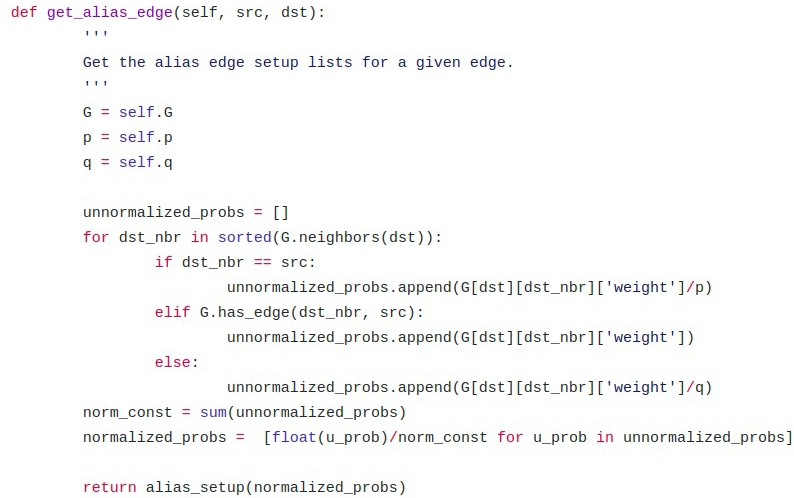
\includegraphics[scale=0.4]{screen-shots/edgelists.jpeg}
        \caption{Random Walk generation}
        \label{fig:my_label}
    \end{figure}
    \FloatBarrier
    \\
The goal of this function is to generate a collection of $\ node IDs $. Firstly, let's consider we are on a random walk and have just transitioned from node $\ dst $ to node $\ src $, however, probability to transition from node $\ src $  to any one of his neighbors node $\ dst$ is edge-weight and $\ \alpha $ (normalized) where $\ \alpha $ is dependent on hyperparameters $\ P $ and $\ Q $. $\ P $ controls the probability to go back to $\ dst $ after visiting $\ src $, while $\ Q $ controls the probability to go explore undiscovered parts of the graphs, where all the unnormalized probabilities are obtained using a normalization constant.

\subsection{Code Snippet on Learn Embeddings}
\begin{figure}[!h]
    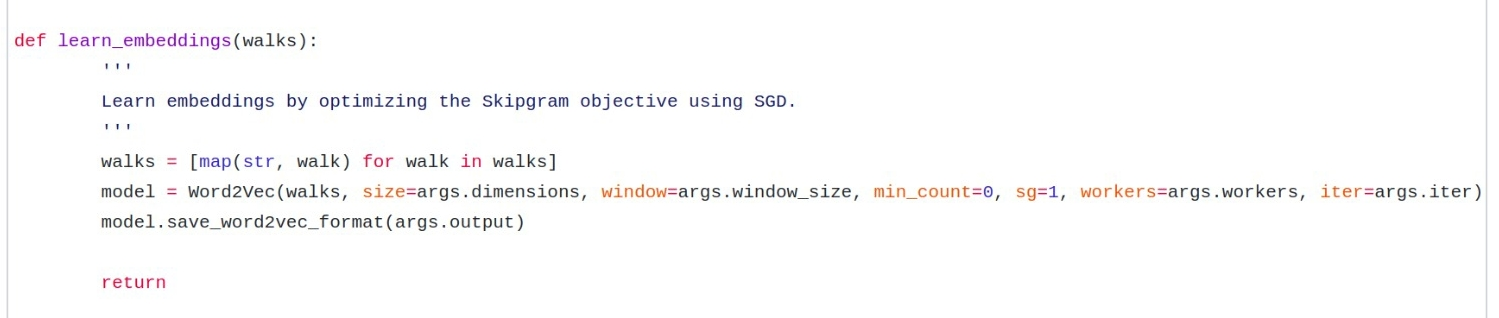
\includegraphics[scale=0.35]{screen-shots/embed.jpg}
    \centering
    \captionof{figure}{Learning embeddings}
	\label{figuur:opnemer}
    
\end{figure}
\FloatBarrier
The goal of the function above is to generate node embeddings by using skip-gram models and Continuous Bag-of-Words model (CBOW). The skip-gram model takes in every $\ node IDs $ i.e. walks, generated by node2vec in the graph and also takes one by one the $\ node IDs $ that surround it within a defined window to then feed a neural network that after training will predict the probability for each $\ node IDs $ to actually appear in the window around the  focus $\ node IDs $.



\section{Walklets}
The \textit{Walklets} approach shares a lot of its root with \textit{Word2Vec}. In fact, \textit{Walklets} use the same objective function as \textit{Skip-grams} algorithm of \textit{Word2Vec} to minimize the probability of predicting a wrong context of vertices while ignoring the order of neighbors. The main difference introduced in \textit{Walklets} is how the walks are generated before the objective function is applied. Therefore, the \textit{Walklets} implementation focuses primarily on generating random walks with a specified number of skipped nodes. Later, these random walks of different \textit{skip-factors} are passed down to \textit{Word2Vec} \textit{Skip-gram} algorithm that computes the embeddings by applying the objective function mentioned above.\\


\subsection{Code Snippet on how Walklets are generated}
    \begin{figure}[h!]
        \center
        {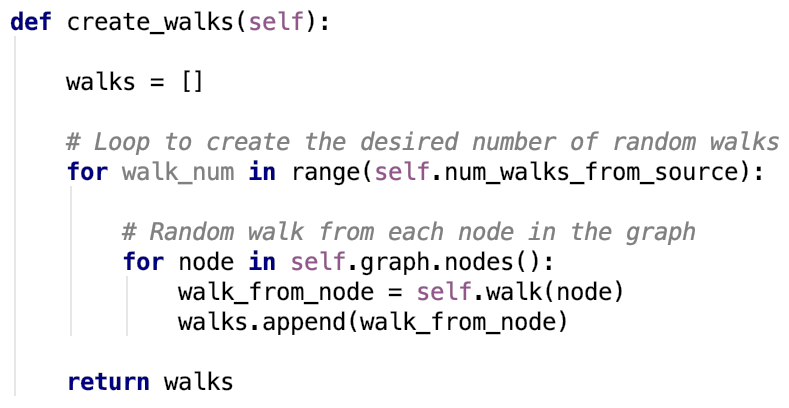
\includegraphics[scale=0.6]{screen-shots/walklets_create_walks.png}}
        \caption{Walklets generation}
        \label{fig:my_label}
    \end{figure}
    \FloatBarrier 

We start creating \textit{Walklets} by generating random walks of specified length from each node in the graph. The outer for-loop will repeat the code as many times as the desired number of random walks from one source. The inner for-loop will perform a random walk of pre-set length from each and every node in the graph.

A walk is performed by simply visiting a node in the graph, and observing its neighbors. If neighbors exist, then one of them is randomly chosen to be added to the walk. The loop moves to the newly added node, and its neighbors and selected. This process continues until the number of nodes in the walk matches the specified length of the walk.

\subsection{Code Snippet on Walklets Representations}
    \begin{figure}[h!]
        \center
         {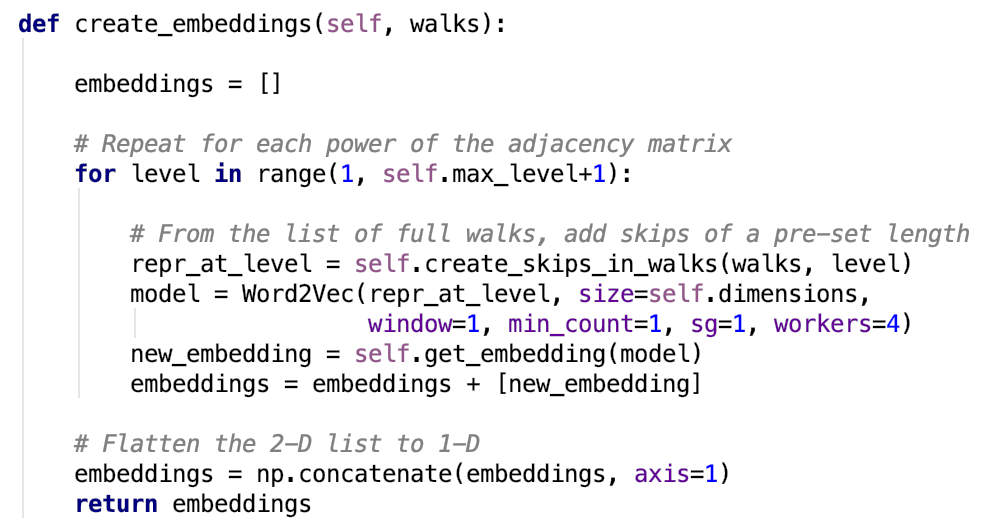
\includegraphics[scale=0.5]{screen-shots/walklets_create_embeddings.png}}
        \caption{Embeddings}
        \label{fig:my_label}
    \end{figure}
    \FloatBarrier
Once the full walks without skips are built, they can be passed down to \textit{create\_embeddings} function. This function will generate embeddings of each independent power of the adjacency matrix representing the graph. As we recall, the power of the matrix will represent how many hops are there between the nodes in the walks. For simplicity, we refer to these powers as \textit{levels} of the network. For each level, the function will take the complete walk from the list of random walks, and select only the nodes that are exactly $k$ hops away from each other. $k$ is referred to as the \textit{skip-factor}, and corresponds to the power of the adjacency matrix, or, in our terms, to the \textit{level} at which the network is to be represented.


\subsection{Code Snippet Based on K-Number of Skips}
    \begin{figure}[h!]
        \center
         {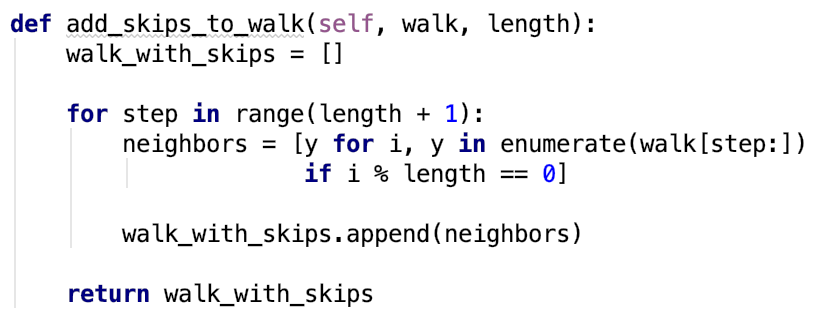
\includegraphics[scale=0.6]{screen-shots/walklets_add_skips.png}}
        \caption{Number of Skip Nodes}
        \label{fig:my_label}
    \end{figure}
    \FloatBarrier

To select the nodes $k$ hops away, we simply enumerate the nodes and select the ones which number is a multiple of $k$. Once the walks in the list are transformed to have the necessary skips, they are passed down to \textit{Word2Vec} algorithm. We set the \textit{sg} parameter to $1$, to specify that we are using the Skip-grams approach. Once embeddings of desired dimensions are created by \textit{Word2Vec}, they are appended to the embeddings list. The list will contain the embeddings for each consecutive power of the adjacency matrix in the ascending order. Flattening this list, we will receive a matrix with the number of rows that is equal to the number of nodes in the graph, and the number of columns that is equal to $\# dimension \times \# levels$. For example, \textit{Walklets} representations for a graph with $5,000$ nodes, $128$ dimensions per representation and $5$ levels of the network will produce a matrix of $5,000 \times 640$ entries.


\section{struc2vec}
Before describing how word2vec of Gensim is used, we start by explaining how to generate the sequences in the random walks file.
\subsection{Generating the sequences}
This section will be dedicated to explain the \textit{struc2vec} code. In what follows we specify the modifications that we have made to the original code in order to adapt it to the provided \textit{"main.py"} file by the tutor. With these interventions, we will get simpler and less complicated code.
\begin{itemize}
\item We removed the function called $parse\_args()$ from the original $"main.py"$ file, which parses the $struc2vec$ arguments. So the input and output files will only be specified in the $"main.py"$ file representing the unified framework. The other arguments were set to their default values and the dimension value was set to 128 as requested.
\item We moved the three functions $read\_graph()$, $learn\_embeddings()$ and $exec\_struc2vec()$ to a single file called $"package\_1.py"$.
\end{itemize}
The two main functions that will help us to generate the embeddings are $learn\_embeddings(input\_file)$ and $exec\_struc2vec(input\_file)$ which are located in the $"package\_1.py"$ file as mentioned previously. In this way, we only need to import the $"package\_1.py"$ file and call the two main functions to generate our embeddings.\\
The execution of $struc2vec$ model is done by the function $exec\_struc2vec(input\_file)$ which is illustrated by the figure \ref{fig:exec}.
\FloatBarrier
\begin{figure}[h!]
  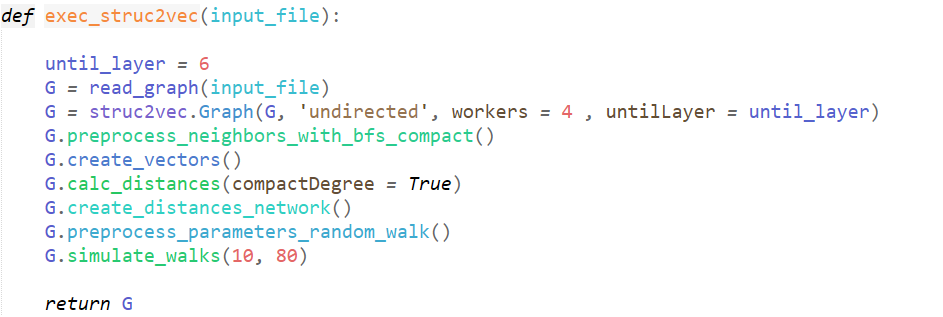
\includegraphics[scale=0.63]{screen-shots/exec.PNG}
  \centering
  \caption{The $exec\_struc2vec$ function}
  \label{fig:exec}
\end{figure}
\FloatBarrier
\\This function is the pipeline for the representational learning for all the nodes in the graph $G$ and it proceeds as follows.
\begin{itemize}
    \item The function $read\_graph(input\_file)$ reads the graph from the $"edgelist"$ file and creates a graph object using the $"Graph"$ class located in the $"struc2vec.py"$ file.
    \item The functions $preprocess\_neighbors\_with\_bfs\_compact()$ and $create\_vectors()$ are responsible for creating the rings of nodes and and the degree sequences denoted by $R_{k}(u)$ and $S(R_{k}(u))$ respectively.
    \item The functions $cal\_distances()$ and $create\_distances\_network()$ are then called to calculate the distance between two nodes.
\end{itemize}
%defined by the following equation:
%\begin{equation}
%f_{k}(u,v) = f_{k-1}(u,v) + g(S(R_{k}(u)),S(R_{k}(v)))  
%\end{equation}
Once the multi-layer graph is constructed, we use the functions $preprocess\_parameters\_random\_walks()$ and $simulate\_walks()$ to perform the random walk and generate the context for a number of walks per node equals $10$ and a walk length equals $80$. This context is a sequence of nodes, instead of words, visited by the random walk and it will be saved in a file called $"random\_walks.txt"$. Consequently, these sequences are going to be used by word2vec of Gensim to learn the embeddings.
 
\subsection{Word2vec of Gensim : Using Skip-gram to learn the embeddings}
Now that we have the $"random\_walks.txt"$ file, we can consider the nodes in this file as words. Thus, we use Skip-gram of word2vec to learn the embeddings while preserving the context relationship, the structural identity of nodes and therefore the similarity between them. To reduce the computational cost of the word2vec model, the authors used Hierarchical Softmax for Skip-gram.
For each node $u$ in the graph, we can learn the latent representation by maximizing the likelihood probability of nodes within the generated context considering a window of size $w=10$ centered around the node. \\
%To achieve that, the Hierarchical Softmax assigns a path on a binary tree of classifiers defined by: $n(u_{i},1), n(u_{i},2), ..., n(u_{i},h)$  where $ n(u_{i},h)$ denotes the leaf node $u_{i}$. 
%In this setting, the likelihood probability can be calculated as follows: 
%\begin{equation}
%P(u_{i}|v_{j}) = \displaystyle\prod_{k=1}^{h} C(n(u_{i},k), v_{j})
%\label{eq2}
%\end{equation}
%where $C$ is a binary classifier present in every node of the binary tree.\\
%Finally, we train Skip-gram considering the likelihood probability as an optimization problem using Stochastic Gradient Decent (SGD). \\
$Word2vec$ is used in the code of the function $learn\_embeddings(input\_file)$ illustrated by figure \ref{fig:learn}.
\FloatBarrier
\begin{figure}[H]
  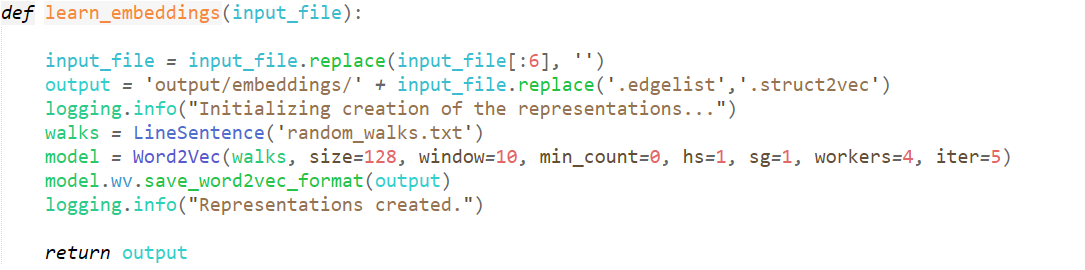
\includegraphics[width=\textwidth, scale=0.7]{screen-shots/lean_emb.PNG}
  \centering
  \caption{The $learn\_embeddings$ function}
  \label{fig:learn}
\end{figure}
\FloatBarrier
The $LineSentence()$ function will iterate over the tokenized sentences or walks contained in $"random\_walks.txt"$ file and we train then our word2vec model. Note that $hs$ (hirarchical softmax) and $sg$ (Skip-gram) are set to $1$ because we are going to use both of them for the training. Moreover, the dimension of the vectors is set to $128$ and the window for the context is $10$.
Finally, we can access the model via the $wv$ attribute and save it to the output file using the $save\_word2vec\_format()$ function.


\section{node2vec with HARP}
\subsection{word2vec as a base to build upon}
Before presenting the proposed implementation, it may be wise to briefly outline some basic notions of Word2vec and to shed some light onto how the considered embedding technique, namely node2vec with HARP, can exploit it. Word2vec comprises 2 algorithms : Continuous Bag Of words (CBOW) and Skip-gram. Both of them are semi-supervised learning techniques from NLP field, where the former, given a context, tries to predict the ‘center word’ and the latter do the exact opposite by predicting a context given a word. Many graph embedding techniques can be implemented by tailoring the original Word2vec to the requirements of graphs data structure.\\ 
Firstly we underlined that the skip-gram is more inline with graphs’ nature simply because it makes more sense to predict a set of nodes when training rather than the opposite. Secondly the training set is build as a sequence of nodes generated according to node2vec’s walking technique. Finally we pass the training set to the word2vec class and since we’re implementing HARP, some changes have to be made to enable the initialization of the neural net with the learned weights in the previous iteration.
\subsection{Key highlights of the proposed implementation}
\subsubsection{main.py file}
In the main.py file we define the function generate\_harp\_embeddings().
the input\_file is the input graph, output\_file is the file where the embedding will be saved, input\_format is the format of the input graph and has ‘edgelist’ as a default value, model is the embedding algorithm to  be assisted by HARP, representation\_size is the dimension over which each node ought to be represented, number\_walks is the number of walks rooting from each node in the graph and walk\_length is the number of nodes in each walk and window\_size defines the number of nodes in the sliding window in skip-gram.
After some initializations  and checkings we pass the previous parameters to geaph\_coarsening.skipgram\_coarsening\_disconnected
where sg=1 means that we want to use skip-gram. This parameter will be passed later to the Word2vec constructor;  hs=0 means that using negative-sampling as activation function in the last layer.

\subsubsection{graph\_coarsening.py file}
In graph\_coarsening.py there are multiple functions but we can not cover all of them due to space constraints. Nevertheless we will present the key functions.
\begin{enumerate}
\item \textbf {external\_ec\_coarsening} function takes the input graph and returns the set of coarsened graphs and the set of recursive merged nodes. The latter is crucial when iterating  over the graphs and initializing the neural nets.

\item \textbf {skipgram\_coarsening\_disconnected} : after some initializations it generates the set of coarsened graphs by calling the previous function and iteratively pass them to Word2vec constructor alongside the parameters that were initially passed in the previous section.

\item \textbf{Word2vec() :} Lastly the core part which consist of calling Word2vec constructor while looping over the coarsened graphs.
\end{enumerate}
\\
\begin{figure}[h!]
    \centering
    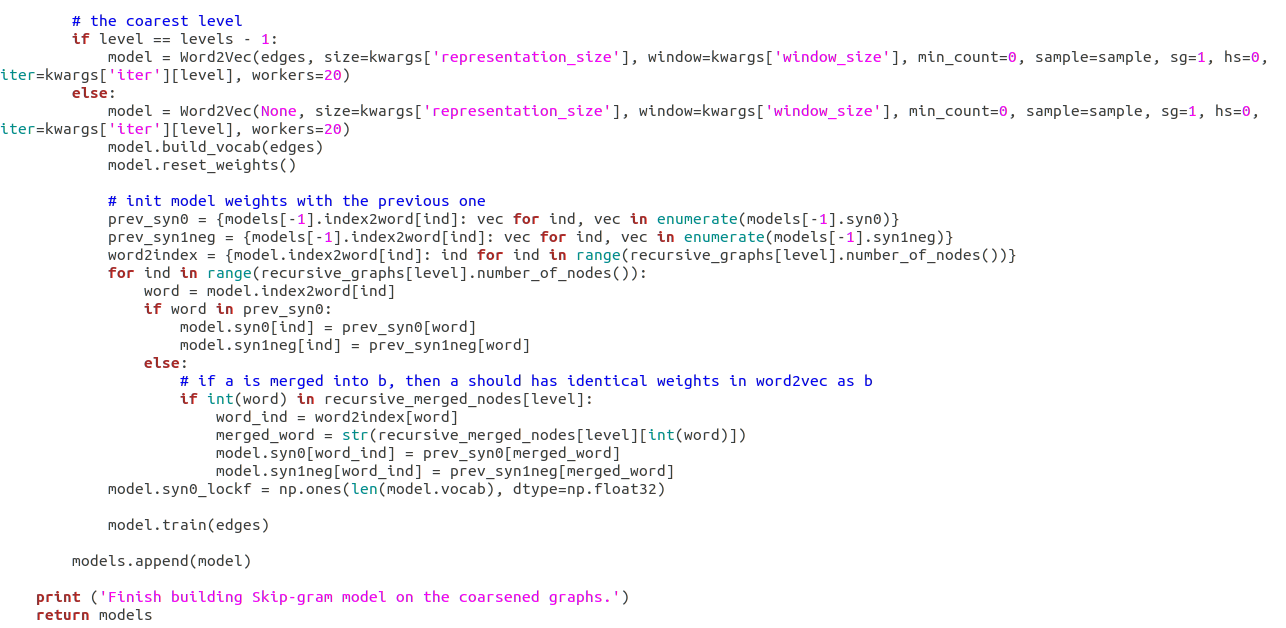
\includegraphics[width=\textwidth]{screen-shots/image2.png}
    \caption{recursive embedding}
    \label{fig:my_label}
\end{figure}
\FloatBarrier
\\
We can see in this part that when iterating over the list of coarsened graphs, we first check : if it is the coarsest graph then we directly pass the training set to Word2vec and the neural net is initialized randomly. If the current graph is not the coarsest one then we initialize the neural net using the weights of the previously trained network. How the initialization is done has been depicted in phase 1.

\section*{Phase(3): Evaluations}
In this sections we will examine the performance of the above mentioned embedding techniques with the help of two evaluation methods, namely : Node classification and link prediction.
\section{Data sets}
\begin{table}[!h]

\caption{\small Statistics of datasets.}
\label{tab:data}
\begin{center}
\small

\begin{tabular}{ccccc}
{\bf Dataset}  & {\bf Nodes } &{\bf Edges } &{\bf Attributes }&{\bf Labels }\Tstrut\\
 \hline 
 \Tstrut
Cora         & 2,708 &  5,429&  1,433 & 7\Tstrut\\
Citeseer      &3,312& 4,660 & 3,703 &  6\Tstrut\\
\end{tabular}
\end{center}
\end{table}

Cora~\cite{citeseer} and Citeseer~\cite{citeseer}:
\begin{itemize}
\item The labels indicate publications topics.
\item Attributes are binary representations of words in the corresponding publications.
\end{itemize}


\section{Node classification}
The idea behind node classification is to assess the quality of the new representation of the data by feeding them into a classifier and examining its performance afterwards. The same idea is prevalent in NLP where word embeddings is fed to an external machine learning task and the quality is assessed according to the performance of the latter. Table 1 states the macro-F1 score of a multi-class linear regression classifier trained over different proportion of the embedded data.



%\begin{figure}[H]
%    \centering
%    \includegraphics[width=17cm]{link_prediction.pdf}
%    \caption{Impact of threshold $\alpha$ on Link Prediction.}
%    \label{fig:my_label2}
%\end{figure}

 
\begin{table}[H]


\begin{center}
\begin{tabular}{cccc ccc ccc cc}
\hline
\textbf{Dataset}&
\textbf{Model}&
\multicolumn{5}{c}{\textbf{Macro-F1} }&

 \Tstrut\\
  \hline  
\Tstrut

  &  & &  $10\%$  &  $30\%$  & $50\%$ &  $70\%$  &$90\%$\Tstrut\\

 \Tstrut
 \multirow{4}{*}{Cora}& HARP &  & \textbf{0.76}  & \textbf{0.80} &\textbf{0.82} &\textbf{0.81} &\textbf{0.82} \Tstrut\\
    &Walklets($A^3$)& &0.73 & 0.78 & 0.79 & 0.80 & 0.81 &\\
    & node2vec & & \textbf{0.76} & 0.78 & 0.80 & 0.80 & 0.78 & \\
     & Struc2vec & & 0.24 & 0.28 & 0.31 & 0.31 & 0.28\\
      \hline 
      
 \Tstrut
 \multirow{4}{*}{Citeseer}& HARP &  &0.48  &\textbf{0.54} &0.55 &\textbf{0.5}6&\textbf{0.56}\Tstrut\\
    &Walklets($A^3$)&  &  0.46 & 0.48 & 0.52 & 0.54 & 0.51 &\\
    & node2vec & & \textbf{0.51} & \textbf{0.54} & \textbf{0.57} & \textbf{0.56}  & 0.52 &\\
     & Struc2vec & & 0.22   & 0.27  & 0.25  & 0.29  & 0.28 \\
     
   


\hline 
   
\end{tabular}
\label{tab:partial}
\end{center}
\caption{Comparison of the baseline methods for node classification.}
\end{table}

\subsection{\textbf{HARP}} For both data sets the performance increases with the proportion of training data but stabilizes after 50\% which means that at this proportion the model already reached its maximum in detecting the  the hidden latent within the data. 
\\
Another expected observation is the relative  improvement over node2vec which was predictable given the fact that HARP acts as a booster or amplifier for the embedding models.  
Lastly the relative difference between the scores on cora and citeseer is mainly due to two reasons:
\begin{itemize}
    \item The inner structure of both graphs: meaning that in cora the information about connections was enough to discriminate the classes whereas it wasn't the case in Citeseer.
    \item Since the connectivity was not enough to discriminate classes other features should have been taken into account to yield better representation. But since the algorithm only considers the connectivity, mediocre results are then completely expected.
\end{itemize}
%\vspace{1cm}
\subsection{\textbf{Struc2vec}}
 We observe that Struc2vec is showing the worst results for both "Cora" and "Citeseer" datasets compared to the other methods as the score does not exceed 30\%. In fact, this is a very interesting result because it reflects the difference between Struc2vec and the other approaches as it mainly focuses on modelling the structural identity of the nodes. However, the labelling of the used datasets in this lab did not account for the role played by the nodes which justifies the low score. For example, if two nodes with labels 0 and 1 respectively play the same structural role in the graph, Struc2vec embeds them together in the same cluster, and this causes an error as some nodes are classified into the wrong cluster because of the obligation of respecting the structural identity. "Cora" dataset is composed of scientific publications classified into 7 labels, these labels do not take into consideration structural roles. So when we run Struc2vec, it will embed together nodes that are structurally similar in the graph regardless of their labels and this can be seen in the visualization results where one cluster can have nodes with different labels. \\
For better explanation of the results of Struc2vec, we consider the "Brazilian air-traffic" dataset, in which labels are more related to the role played by the airport (for example label 1 is given to the 25\% less active airports etc.). By using Struc2vec on this dataset, we obtain scores of more than 80\% for node classification.

\subsection{\textbf{node2vec}}

In the node classification setting, every node is assigned one or more labels. During the training phase, we observe the nodes and all their labels. We utilize the following two datasets:
\begin{itemize}
\item Citeseer 
\item Cora
\end{itemize}
These networks datasets exhibit a fair mix of $ homophilic \ $ and $ structural \ $ equivalences. 
The train and test data is split equally over some random instances. We use the $ Macro-F1 \ $ score for comparing performance in $ Table 1 \ $  and the relative performance gain is over the closest benchmark. From the results, it is evident, we can see how the added flexibility in exploring neighborhoods allows $ node2vec \ $ to outperform the other benchmark algorithms except $ HARP \ $ which combines $ node2vec \ $ during the embedding process. For the $ Cora \ $  $ dataset \ $, we can discover the right mix of $ homophily \ $ and $ structural \ $ equivalence by setting parameters $ p \ $ and $ q \ $ to default values, giving us a bit edge of performance over $ Struc2vec \ $ and $ walklets \ $.  
For a more fine-grained analysis, we also compare performance while varying the train-test split from \%10 to \%90 while learning parameters $ p \ $ and $ q \ $ on \%10 of the data as before. 
We summarize the results for the Macro-F1 scores graphically in Table 1.

\subsection{\textbf{Walklets}}
As \textit{Walklets} capture the \textit{Skip-gram} representation of the network on different independent levels by introducing skips in random walks, we first have to determine which of the representations $A^1$, $A^2$, $A^3$ fits best the classification task. For both of these datasets the coarse representation $A^3$ demonstrated the best results. Since the labels in the dataset are classes defined by broader publication topics, our expectations held true, that the representation of a higher level of this network will suit better for this task.

Comparing the results to other methods, we observed that the coarse representation of the network \textit{Walklets} in several cases yielded similar results as in \textit{node2vec}. We explain this observation by the fact that the preset parameters in \textit{node2vec} ($P$ and $Q$) were also targeting a more global representation of the network. Analogously, we observe that \textit{Walklets} performed significantly better than \textit{struc2vec}, which demonstrates us that neighborhood associations of the nodes are still preserved, even if the representation is learned from a higher level of the network by the method of skipping nodes in random walks.






\bigbreak

\section{Link prediction}
With link prediction we mainly want to test if the new representation is able to catch the first-order proximity in the original graph. Hence 50\% of edges will be randomly deleted from the input graph and the remaining edges constitutes the set of positive instances while the same amount of negative instances will be generated by randomly sampling disconnected node pairs from the original graph. A logistic regression model will trained and evaluated on these data. Table 2 depicts the AUC for the 4 algorithms using Hadamard and Average aggregation functions.

\begin{table}[H]

    \begin{center}
\begin{tabular}{cccc ccc ccc cc}
\hline
\textbf{Dataset}&
\textbf{Method}&
\multicolumn{4}{c}{\textbf{AUC} }& \Tstrut\\
  \hline  
\Tstrut
\Tstrut
  &  & \textbf{Hadamard}  &  \textbf{Average} & \textbf{L1} & \textbf{L2} &  \Tstrut\\

 \multirow{5}{*}{Cora}&node2vec & 0.993 &\textbf{0.834} & \textbf{0.997} & \textbf{0.997} &\Tstrut\\
   & Walklets($A^2$)  & 0.990 &  0.778 & 0.908 & 0.911 &\Tstrut\\
   & HARP(node2vec)  &\textbf{0.997} &0.744 & \textbf{0.997} & \textbf{0.997} &\Tstrut\\
   & Struc2vec & 0.6503 & 0.6569 & 0.6204 & 0.6213 & \Tstrut\\
     \hline 
     
      \Bstrut
  \multirow{5}{*}{Citeseer}&node2vec  & 0.993 &0.716& 0.994 & 0.993 &\Tstrut\\
   &  Walklets($A^2$)  & 0.993& \textbf{0.861} & 0.915 & 0.922 &\Tstrut\\
    &  HARP(node2vec)  & \textbf{0.995} & 0.0682& \textbf{0.997} & \textbf{0.996} &\Tstrut\\
  &  Struc2vec  &  0.8067  & 0.6685 & 0.7069 & 0.7232 &\Tstrut\\
   
    
  \hline 
\end{tabular}
\label{tab:partial}
\end{center}
\caption{ Link prediction performance (AUC) of different methods on different datasets.}
\end{table}
\bigbreak
\subsection{\textbf{HARP}}
The main takeaways from the above results are:
\begin{itemize}
    \item Node2vec assisted with HARP is indeed able to maintain the first order proximity which is reflected in 0.99 AUC score on both data sets.
    \item We also can notice the expected improvement over node2vec.
\end{itemize}
\subsection{\textbf{Struc2vec}}
We notice that Struc2vec gives lower results than other methods. It is explained by the fact that it focuses on modelling the structural identity of the nodes. Besides, Struc2vec is more suitable for larger scale graphs with different layers, because it creates a multi-layer graph. This hierarchical architecture incorporates nodes degree distributions from the bottom as well as the top of the graph. Therefore, an embedding technique that accounts for the multi-layer existence and interaction of nodes will equip the learning algorithm with a richer vocabulary for learning tasks like link prediction across the different networks.

\subsection{\textbf{node2vec}}
Considering the result for link prediction, we summarize our results for link prediction in $ Table 2 \ $.  For a general observation, what we can draw from the results is that, the learned feature
representations for node pairs, where $ node2vec \ $ significantly outperform the $ struc2vec \ $ and $ walklets \ $ with some margins approximately \%0.30.
However, benchmark scores for $ HARP \ $ is achieving the best $ AUC \ $ improvement about \%0.40 on the $ Cora \ $  Dataset over the best performing $ node2vec \ $. Nevertheless, $ HARP \ $ is embarked by $ node2vec \ $ algorithm.
$ node2vec \ $ outperforms $ walklets \ $ and $ struc2vec \ $ in a couple of cases involving the Weighted-L1 and Weighted-L2 operators in which $ HARP \ $ performs better. Overall, the $ Hadamard \ $ operator when used with $ node2vec \ $ is highly stable and gives the best performance on average across all networks.

\subsection{\textbf{Walklets}}
Reviewing the \textit{Walklets} results for the link prediction task, we once again compared the scores for the representations of each level of the network $A^1$, $A^2$, $A^3$ to analyze which one yields better results. For this particular task the \textit{medium} scale $A^2$ slightly outperformed the others. We did not expect a coarse representation to perform well, because if a node is skipped in a random walk (which is the case of any $A^k$ where $k>1$, it may not capture correctly the edge between two particular nodes, and will score lower in link prediction, when compared to the original graph. Depending on the structure of the graph, and configurations for random walks, the walk may still come back to the original neighbors of the source node, and we believe this factor allows us to see reasonable results even when using higher skip-factors $k>1$ and learning higher level representations of the network.

\section{Visualization}
%\subsection{Cora visualization}

In figure \ref{fig:myfig}, we can observe that the good scores of node2vec, HARP(node2vec) and Walklets are reflected in the visualizations since they place nodes from the same class near each other in the embedding space. Furthermore, we can also see that node2vec and HARP(node2evc) were able to capture some kind of dense region that Walklets was unable to, which explains why the scores of the formers are better than the latter. \\
As for Struc2vec, the visualization in figure \ref{fig:d} confirms the low node classification scores as there are many nodes with different labels within the same cluster. These nodes, according to Struc2vec, have the same structural role in the graph regardless of their labels. Therefore, the node classification evaluation results for Struc2vec will be low. 

\begin{figure}[H]
\centering
\subfloat[\normalsize Node2vec ]{\label{fig:a}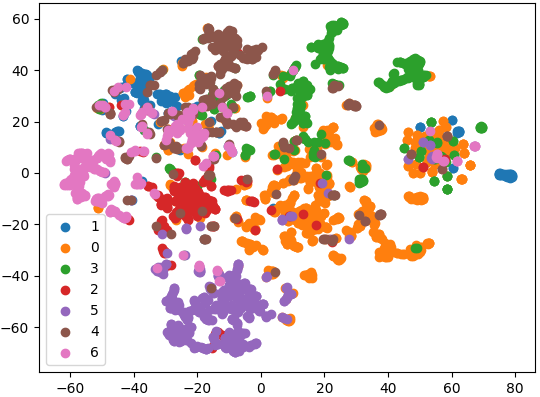
\includegraphics[width=0.45 \linewidth]{screen-shots/Node2vec_cora}}\qquad
\subfloat[\normalsize Harp (Node2vec)]{\label{fig:b}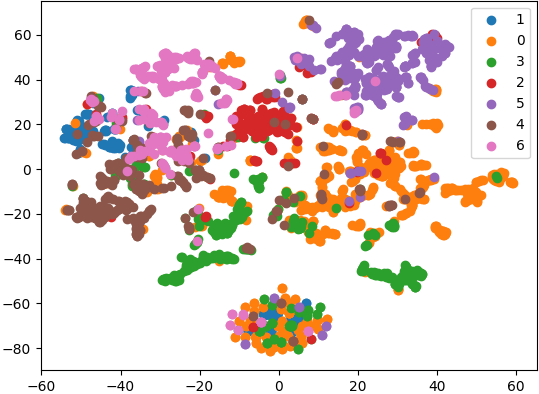
\includegraphics[width=0.45 \linewidth]{screen-shots/harp_cora}}\\
\subfloat[\normalsize Walklets $(A^2)$]{\label{fig:c}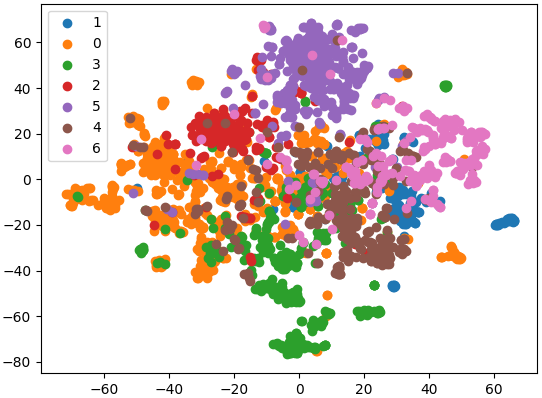
\includegraphics[width=0.45 \linewidth]{screen-shots/Walklets_k2_cora.png}}\qquad%
\subfloat[\normalsize Struc2vec]{\label{fig:d}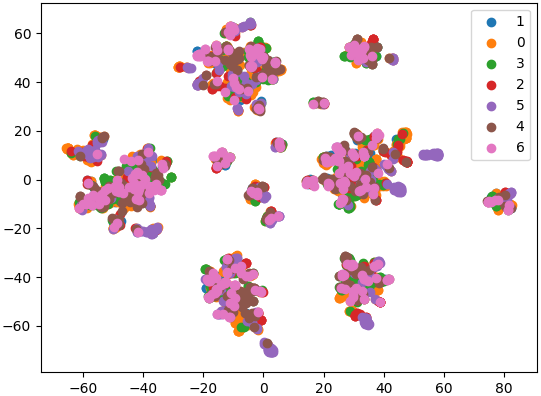
\includegraphics[width=0.45 \linewidth]{screen-shots/cora_struc.png}}%
\vspace{5mm}
\caption{\normalsize Visualization of the 4 embedding methods for the Cora dataset}
\label{fig:myfig}
\end{figure}
\FloatBarrier

\begin{thebibliography}{9}

\bibitem{deepwalk}
Perozzi, B., Al-Rfou, R., and Skiena, S. 2014. "Deepwalk: Online learning of social representations." In Proceedings of the 20th ACM SIGKDD international conference on Knowledge discovery and data mining, 701–710. ACM.

\bibitem{node2vec}
Grover, Aditya, and Jure Leskovec. "node2vec: Scalable feature learning for networks." In Proceedings of the 22nd ACM SIGKDD international conference on Knowledge discovery and data mining, pp. 855-864. ACM, 2016.

\bibitem{walklets}
Perozzi, Bryan, Vivek Kulkarni, and Steven Skiena. "Walklets: Multiscale graph embeddings for interpretable network classification." arXiv preprint arXiv:1605.02115 (2016).

\bibitem{struc2vec}
Ribeiro, Leonardo FR, Pedro HP Saverese, and Daniel R. Figueiredo. "struc2vec: Learning node representations from structural identity." In Proceedings of the 23rd ACM SIGKDD International Conference on Knowledge Discovery and Data Mining, pp. 385-394. ACM, 2017.

\bibitem{harp}
Chen, Haochen, Bryan Perozzi, Yifan Hu, and Steven Skiena. "Harp: Hierarchical representation learning for networks." In Thirty-Second AAAI Conference on Artificial Intelligence. 2018.
 
\bibitem{citeseer} Prithviraj Sen, Galileo Namata, Mustafa Bilgic, Lise Getoor, Brian Gal-
ligher, and Tina Eliassi-Rad, "Collective classification in network data",
AI magazine, 29(3), 93-93, (2008).

\bibitem{fb} Jure Leskovec and Julian J Mcauley, "Learning to discover social circles in ego networks", in Advances in neural information processing
systems, pp. 539-547, (2012).
\end{thebibliography}

%\bibliographystyle{IEEEtran}

%\bibliography{svd-pairwise}


\end{document}
